%%=============================================================================
%% Methodologie
%%=============================================================================

\chapter{\IfLanguageName{dutch}{Methodologie}{Methodology}}%
\label{ch:methodologie}

% Door de vergaarde kennis uit de literatuurstudie in hoofdstuk \ref{ch:stand-van-zaken} over de mogelijke noden van scholieren met dyslexie, de complexiteit van wetenschappelijke artikelen, de technieken voor MTS en ATS, en de bijhorende valkuilen bij taalverwerking met AI, kunnen onderzoeksmethoden worden toegepast om een antwoord te vinden op de onderzoeksvraag. 

Hiervoor moeten drie onderzoeksmethoden toegepast worden, met als hoofddoel het ontwikkelen van een prototype voor gepersonaliseerde ATS om wetenschappelijke artikelen te vereenvoudigen voor scholieren met dyslexie in de derde graad van het middelbaar onderwijs.

\section{Requirementsanalyse}
\label{sec:requirementsanalyse}

Om de ontwikkeling van het prototype zo gefocust te laten verlopen, moet het onderzoek stilstaan bij de toegepaste MTS en ATS technieken bij bestaande tools. Dit gebeurt door middel van een requirementsanalyse. Met een verkennend onderzoek en korte experimenten bouwt deze onderzoeksfase een Moscow-schema op met de nodige functionaliteiten voor ATS, met evenwaardige capabiliteiten als die van gepersonaliseerde MTS. De geteste toepassingen opgesomd in \ref{table:shortlist-tools} representeren de \textit{top-of-the-line} toepassingen voor (gepersonaliseerde) ATS. Zo omvat deze lijst zowel erkende toepassingen van de overheid, alsook toepassingen die leerkrachten of scholieren kunnen gebruiken om teksten te vereenvoudigen. Met deze onderzoeksmethode kan het onderzoek een antwoord geven op de volgende twee deelvragen van het onderzoek:

\begin{itemize}
	\item Welke functies ontbreken AI-toepassingen om geautomatiseerde tekstvereenvoudiging mogelijk te maken voor scholieren met dyslexie in de derde graad middelbaar onderwijs?
	\item Welke manuele methoden voor tekstveree²nvoudiging komen niet in deze tools voor?
\end{itemize}

\medspace

Zoals aangewezen in sectie \ref{sec:beschikbare-tools-en-taalmodellen}, beschikken scholen over vijf door de overheid erkende softwarepakketten, maar de requirementsanalyse betrekt enkel drie van deze vijf, omwille van hun prevalentie in het onderwijs en de functionaliteiten die de literatuurstudie eerder uitwees. Daarnaast kunnen online beschikbare tools ook scholieren met dyslexie ondersteunen bij het intensief lezen van wetenschappelijke artikelen met ATS, zoals bewezen in \textcite{Bingel2018}. De requirementsanalyse betrekt enkel tools met onderschreven tekstvereenvoudigingscapaciteiten en laat daarmee pure samenvattingstools erbuiten. Tabel \ref{table:shortlist-tools} geeft een overzicht weer van de tools waarvan het onderzoek experimenten op uitvoert.

\begin{center}
	\begin{table}[H]
		\begin{tabular}{ | m{6cm} | m{6cm} | } 
			\hline
			\textbf{Erkende software} & \textbf{Online beschikbare tools} \\
			\hline
			Sprintplus & Simplish \\
			Kurzweil3000 & SciSpace \\ 
			AlineaSuite & ChatGPT \\
			& Bing Chat\\
			\hline
		\end{tabular}
		\caption{Shortlist van uit te testen tools en toepassingen voor tekstvereenvoudiging.}
		\label{table:shortlist-tools}	
	\end{table}
\end{center}

De eerder genoemde MTS-technieken uit tabellen \ref{table:manual-simplification} en \ref{table:scientific-paper-struggles} vormen de bouwstenen voor het valideren van de functionaliteiten van de tools op de shortlist, met als doel de bruikbaarheid te beoordelen voor gepersonaliseerde ATS in het onderwijs, in het bijzonder voor scholieren met dyslexie in de derde graad van het middelbaar onderwijs. Met behulp van de criteria beschreven in tabel \ref{table:criteria-requirementsanalysis}, experimenteert deze onderzoeksfase met de toegelichte tools om de toegepaste en ontbrekende MTS-technieken in de tools te achterhalen, alsook of deze tools in staat zijn om wetenschappelijke artikelen te kunnen vereenvoudigen. Een verkenning in de tool leidt tot de ontdekking van de verschillende functionaliteiten, waarbij alle aangeboden functies in deze onderzoeksfase aan bod komen.

\begin{center}
	\begin{table}[H]
		\begin{tabular}{ | m{4cm} | m{11cm} | } 
			\hline
			\textbf{MTS techniek} & \textbf{Functionaliteit} \\
			\hline
			Lexicale vereenvoudiging & Rekening houden met doelgroep buiten vakgebied door eenvoudigere synoniemen te schrijven \\
			& Woorden met minder lettergrepen gebruiken \\
			& Extra uitleg schrijven bij zinnen \\
			& Paragrafen herschrijven zodat ze eerst uitleg geven op een high-level niveau, vervolgens lagen van complexiteit toevoegen om de lezer te begeleiden \\
			& Woordenlijst aanmaken \\
			& Synoniemenlijst aanmaken \\
			& Idiomen vervangen door eenvoudigere synoniemen \\
			\hline
			Syntactische vereenvoudiging & Zinnen inkorten \\
			& Verwijswoorden aanpassen \\
			& Voorzetseluitdrukkingen \\
			& Samengestelde werkwoorden aanpassen \\
			& Actieve stem toepassen \\
			& Onregelmatige werkwoorden gebruiken \\
			\hline
			Structurele aanpassingen & Achtergrondkleur aanpassen \\
			& Woord- en karakterspatiering \\
			& Consistente lay-out \\
			& Duidelijk zichtbare koppenstructuur \\
			& Huidige positie benadrukken \\
			& Waarschuwingen geven omtrent formulieren en sessies \\
			& Inhoud visueel groeperen \\
			& Tekst herschrijven als tabel \\
			& Tekst herschrijven als opsomming \\
			\hline
		\end{tabular}
		\label{table:criteria-requirementsanalysis}	
		\caption{Criteria waarop toepassingen worden afgetoetst in de requirementsanalyse}
	\end{table}
\end{center}

\medspace

De requirementsanalyse past de flowchart weergegeven in figuur \ref{img:flowchart-requirementsanalyse} toe.

\begin{figure}
	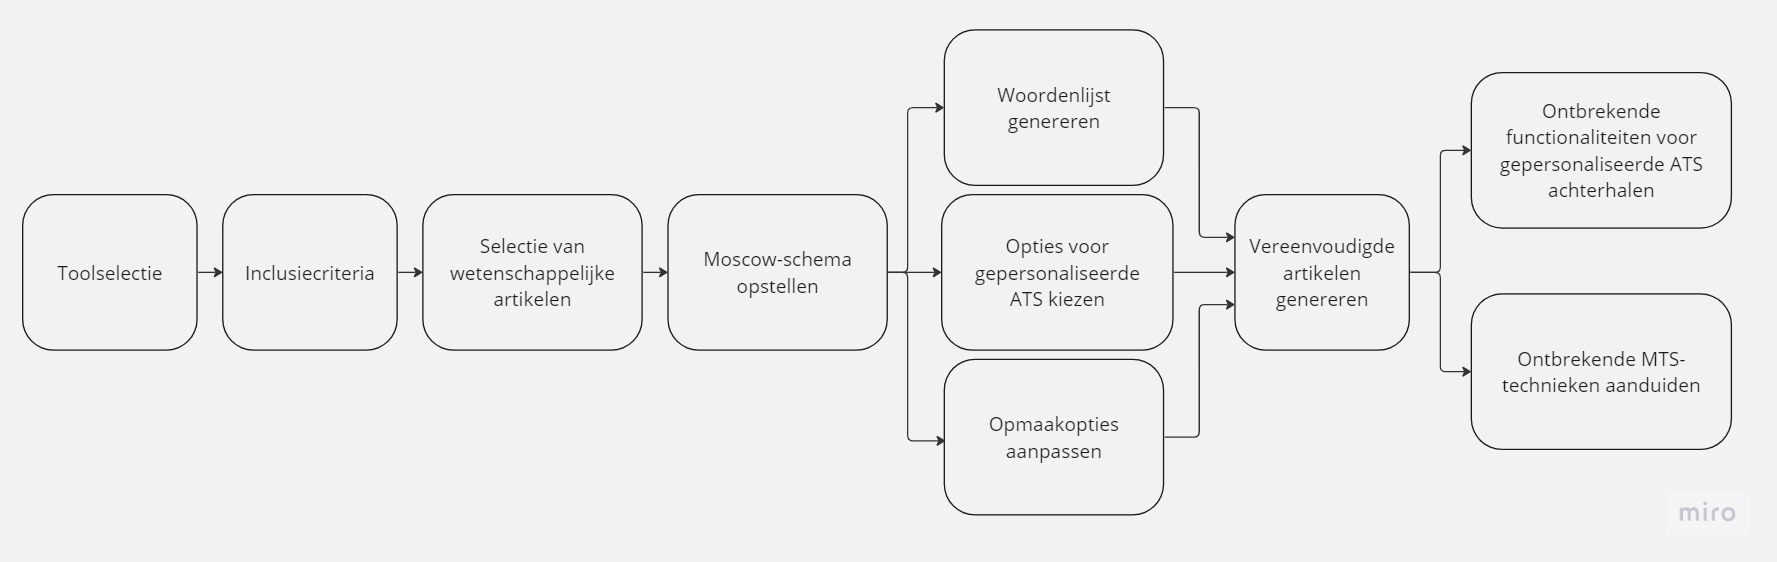
\includegraphics[width=\linewidth]{img/flowchart-requirementsanalyse.jpg}
	\label{img:flowchart-requirementsanalyse}
	\caption{Het toegepaste stappenplan bij de requirementanalyse.}
\end{figure}}

Het uploaden van wetenschappelijke artikelen gebeurt bij SprintPlus, Kurzweil3000, AlineaSuite, Simplish en SciSpace met een PDF-upload, in tegenstelling tot Bing Chat en ChatGPT waarbij PDF-upload niet mogelijk is. Bij deze twee chatbots gebeurt de invoer met \textit{plain-text} of per link. Teksten extraheren gebeurt manueel en dient nadien als invoer voor de chatbot. Beide chatbots krijgen dezelfde tekst voorafgaand van een prompt. Met vijf verschillende prompts kan het onderzoek de capabiliteit om lexicale, syntactische of structurele aanpassingen aan een tekst te achterhalen. Deze prompts staan vermeld in \ref{table:tested-prompts-requirementsanalysis}. 

\medspace
  
Tijdens het experiment krijgen de chatbots eerst een link naar het wetenschappelijk artikel mee, zoals aangegeven in figuur \ref{img:tryout-bing-ai}. Als dit de capabiliteiten van de chatbot overstijgt, dan krijgt de chatbot de tekstinhoud van het wetenschappelijk artikel als \textit{plain-text} mee. Vijf verschillende prompts, weergegeven in tabel \ref{table:tested-prompts-requirementsanalysis}, testen uit welke technieken van lexicale en syntactische vereenvoudiging of structurele aanpassingen deze chatbots kunnen uitvoeren. 

\medspace

Met de huidige erkende softwaretools in het onderwijs is het moeilijk om syntactische vereenvoudiging toe te passen op wetenschappelijke artikelen. Online webtoepassingen bieden weliswaar mogelijkheden om de moeilijkheidsgraad van de zinsstructuur te verlagen, maar ze zijn voornamelijk gericht op het verkorten van de oorspronkelijke tekst, of het maken van een samenvatting. Het aanpassen van tangconstructies, verwijswoorden, voorzetseluitdrukkingen, samengestelde werkwoorden en onregelmatige werkwoorden blijft daarom een uitdaging voor deze toepassingen. Zelfs het schrijven in de actieve stem kan problematisch zijn, en de beschikbare prompts zijn beperkt tot vooraf gedefinieerde transformaties.

\medspace

\begin{figure}[H]
	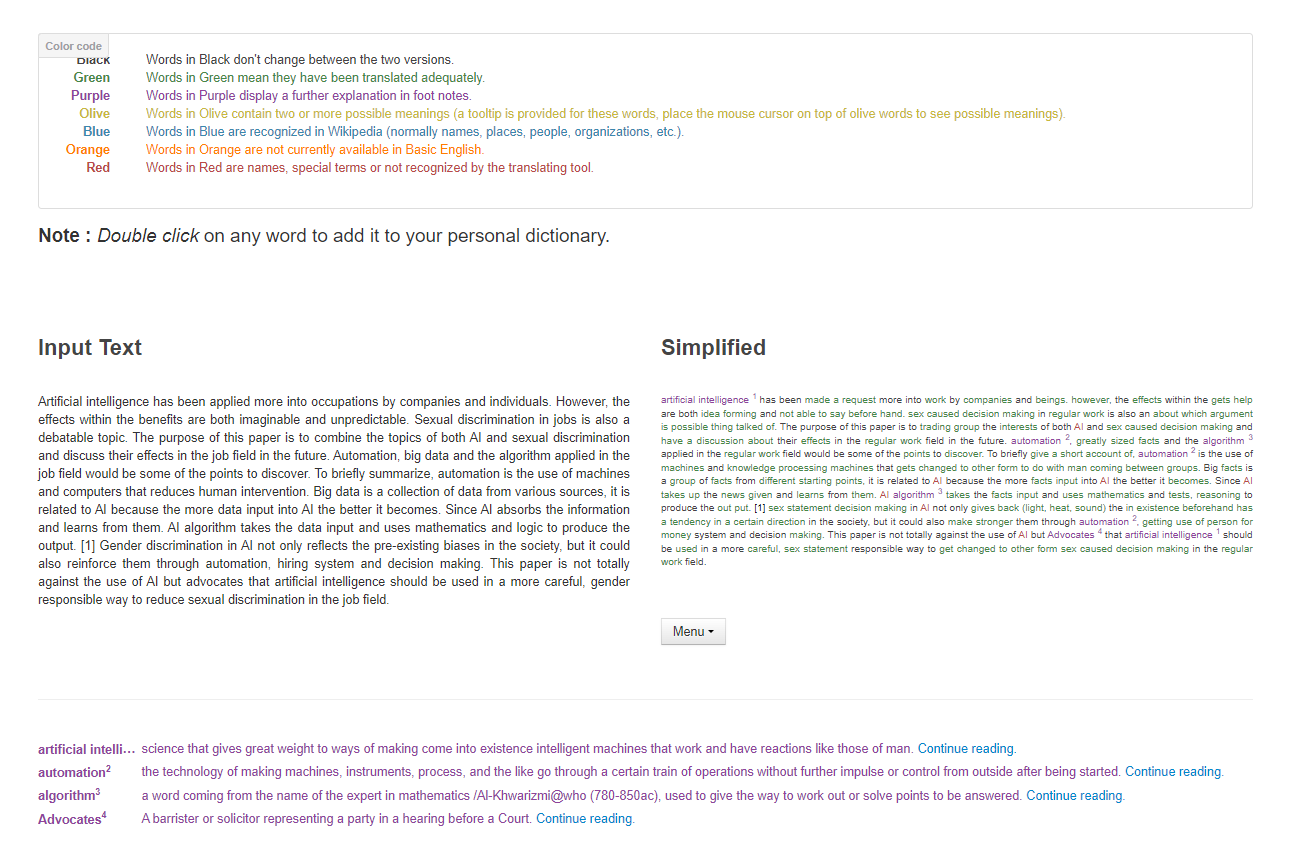
\includegraphics[width=\linewidth]{img/simplish-output.png}
	\caption{Illustratie van de tekstanalyse bij Simplish na een tekstvereenvoudiging.}
	\label{img:simplish-output}
\end{figure}

\begin{figure}[H]
	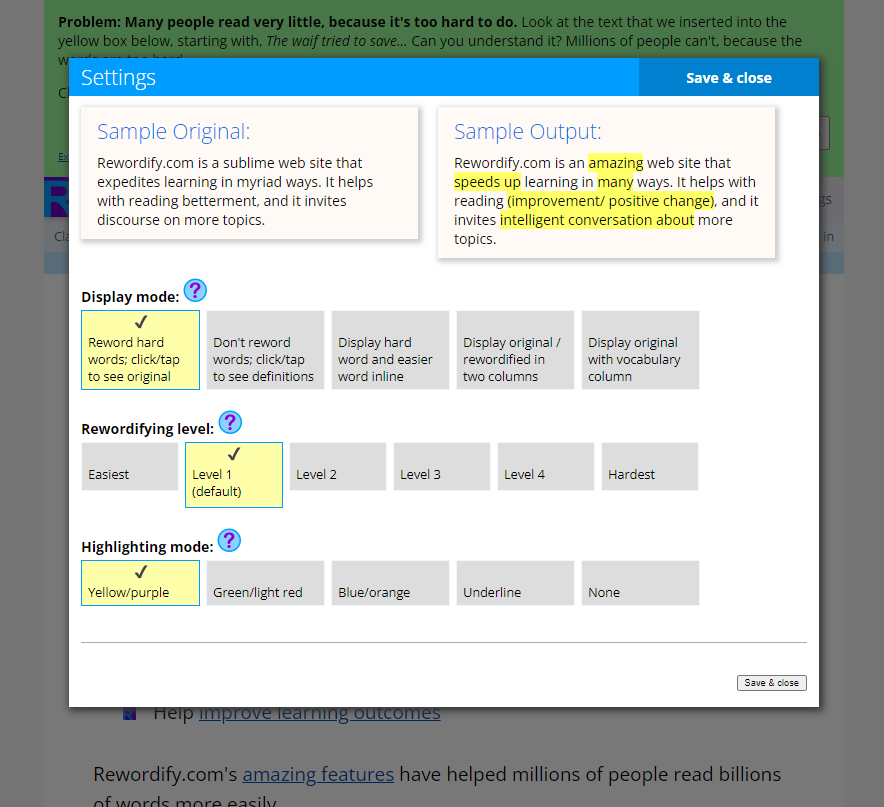
\includegraphics[width=\linewidth]{img/scholarcy-attempt.png}
	\caption{Illustratie van de tekstanalyse bij Rewordify.}
	\label{img:scholarcy}
\end{figure}

% De requirementsanalyse neemt geen functionaliteiten op van obscure proof-of-concepten. Deze ontbreken de nodige testen en zekerheid dat deze effectieve gepersonaliseerde en geautomatiseerde tekstvereenvoudiging aanbieden. Twee van de online tools, namelijk Resoomer en Scispace, bieden uitsluitend samenvattingsfunctionaliteiten aan. Resoomer is sneller geneigd om de belangrijkste zinnen te markeren en vervolgens deze in een kortere tekst terug te geven. Dit kan een effect hebben op de betrouwbaarheid van de functionaliteiten, alsook op de leesgraadmetrieken.

\begin{figure}[H]
	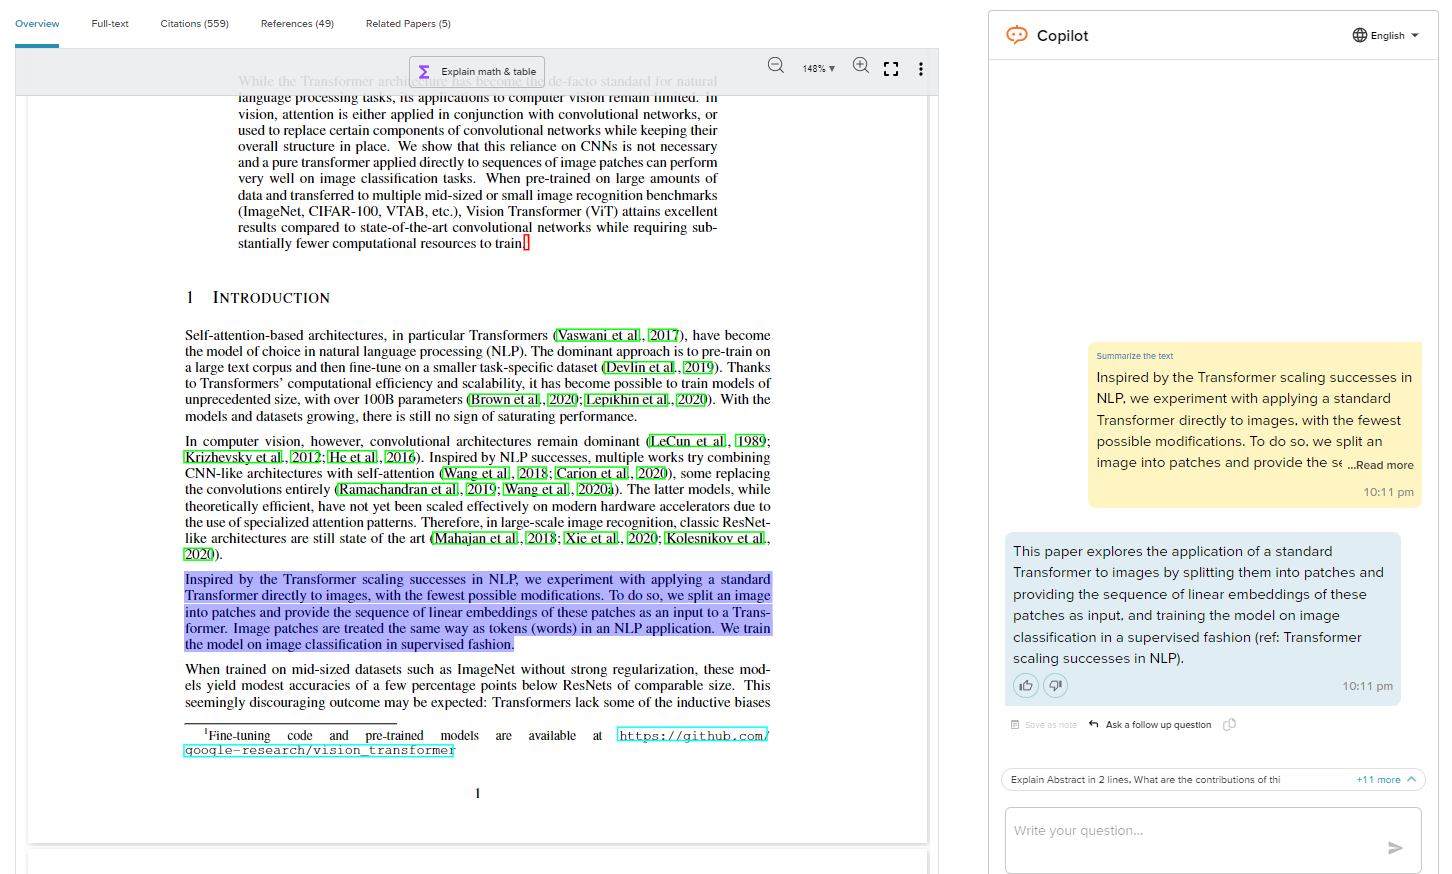
\includegraphics{img/typeset-example.png}
	\caption{Schermafbeelding van SciSpace}
	\label{img:scispace-example}
\end{figure}

\begin{center}
	\begin{table}[H]
		\begin{tabular}{ | m{2cm} | m{14cm} | } 
			\hline
			\textbf{Naam} & \textbf{Prompt} \\
			\hline
			P1 & Vereenvoudig deze tekst \\
			\hline
			P2 & Vereenvoudig deze tekst voor studenten (16-18 jaar) door moeilijke woorden te vervangen, vakjargon te schrappen, woorden langer dan 18 letters te vervangen, acroniemen voluit te schrijven, een woord slechts eenmaal door een synoniem te vervangen, korte uitleg te geven wanneer dat nodig is, en percentages te vervangen. \\
			\hline
			P3 & Vereenvoudig een tekst door deze op te delen in kortere zinnen van maximaal tien woorden. Verander voornaamwoorden als 'zij', 'hun' of 'hij' in namen. Vervang complexe zinsconstructies en voorzetselzinnen door eenvoudiger alternatieven, maar laat ze ongewijzigd als er geen eenvoudiger optie beschikbaar is. \\
			\hline
			P4 & Schrijf de tekst als opsomming. \\
			\hline
			P5 & Schrijf de tekst in tabelformaat. \\
			\hline
		\end{tabular}
		\label{table:tested-prompts-requirementsanalysis}
		\caption{De toegepaste GPT-3-prompts in de requirementsanalyse.}
	\end{table}
\end{center}

\begin{figure}[H]
	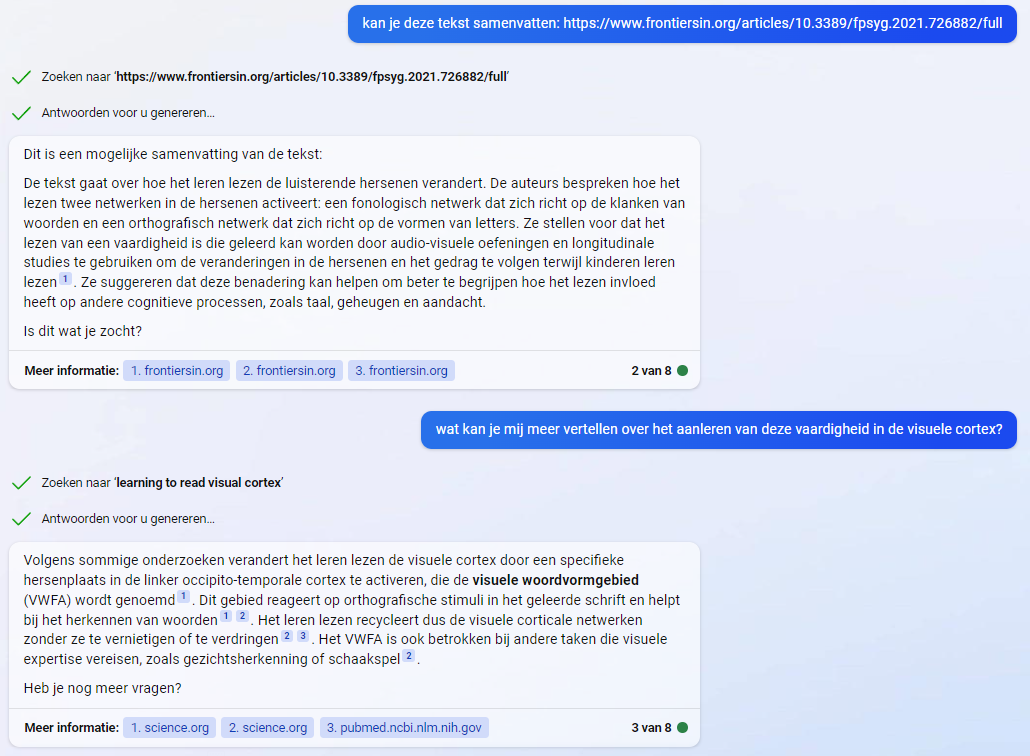
\includegraphics{img/bing-ai-chatbot-example.png}
	\caption{Resultaat Bing Chat}
	\label{img:tryout-bing-ai}
\end{figure}

\medspace


Deze experimenten resulteren in een Moscow-schema die fungeert als bouwsteen voor de ontwikkeling van het prototype voor gepersonaliseerde ATS van wetenschappelijke artikelen, specifiek op maat voor scholieren met dyslexie in de derde graad van het middelbaar onderwijs. 

\medspace

\begin{center}
	\begin{table}

	\begin{tabular}{ | m{4cm} | m{12cm} | } 
		\hline
		\textbf{MoSCoW-principe} & Functionaliteit \\
		\hline
		Must-have & Gepersonaliseerde vereenvoudiging aanbieden, waaronder lexicale en syntactische vereenvoudiging aanbieden, na het toevoegen van een respectievelijke API-sleutel. \\
		& Wetenschappelijke artikelen in PDF-vorm opladen. \\
		& Formaatwijzigingen toepassen aan de oorspronkelijke tekst. \\
		& Personaliseerbare toepassing: lettertype -en grootte aanpassen, tekstformaat aanpassen, achtergrondkleur aanpassen \\
		& Lokale opzet \\
		\hline
		Should-have & Glossary genereren na handmatige selectie van moeilijke woorden \\
		& Personaliseerbare PDF- of Worddocumentlay-out \\
		& Uitvoer als PDF of Word-bestand teruggeven. \\
		& Tekstanalyse voor en na de vereenvoudiging aanbieden. \\
		\hline
		Could-have & Glossary genereren na automatische selectie van moeilijke woorden \\
		\hline
		Wont-have & Beschikbaarheid tot de tool zonder Docker Desktop, in de vorm van online webtoepassing of browserextensie. \\
		& Beschikbaarheid tot de standaard- en gepersonaliseerde opties zonder API-sleutels \\
		\hline
	\end{tabular}
	\label{img:moscow-table}
	\caption{Het Moscow-schema, opgebouwd door middel van de requirementsanalyse.}
	\end{table}
\end{center}




\section{Vergelijkende studie}
\label{sec:vergelijkende-studie}

Teksten vereenvoudigen met ATS kan niet efficiënt verlopen zonder een taalmodel, maar een toepassing voor tekstvereenvoudiging binnen de casus van wetenschappelijke artikelen moet gebruik maken van een taalmodel die het meest aansluit op deze casus. Om het prototype af te stemmen op één taalmodel, vereist er een antwoord op de volgende vraag. 

\begin{itemize}
	\item Welk taalmodel of LLM is geschikt voor ATS van wetenschappelijke artikelen voor scholieren met dyslexie in de derde graad van het middelbaar onderwijs, met dezelfde of gelijkaardige kwaliteiten als gepersonaliseerde tekstvereenvoudiging met MTS?
\end{itemize}


Gezien de schaarse hoeveelheid aan gespecialiseerde taalmodellen, specifiek gericht op het vereenvoudigen van wetenschappelijke artikelen of taalmodellen met een personaliseerbaar karakter, beoordeelt de vergelijkende studie alle vermelde taalmodellen die speicifiek op ATS gericht zijn, beschreven in \ref{table:huggingface-models}. 

\begin{center}
	\begin{table}[H]
		\begin{tabular}{ | m{4cm} | m{12cm} | } 
			\hline
			\textbf{Verwijzing} & \textbf{Taalmodel} \\
			\hline
			T1 & Haining Scientific Abstract Simplification\footnote{https://huggingface.co/haining/scientific\_abstract\_simplification} \\
			\hline
			T2 & Keep It Simple\footnote{https://huggingface.co/philippelaban/keep\_it\_simple} \\
			\hline
			T3 & \\
			\hline
			T4 & GPT-3 \\
			\hline
		\end{tabular}
		\caption{Gebruikte taalmodellen in de vergelijkende studie}
		\label{table:vergelijkende-studie-taalmodellen}
	\end{table}
\end{center}

\medspace

Zo vergelijkt deze onderzoeksfase de leesgraadsmetrieken van de oorspronkelijke wetenschappelijke artikelen zoals in \ref{sec:requirementsanalyse}, met referentieteksten vereenvoudigd via MTS en teksten vereenvoudigd met ATS. Zinnen worden vereenvoudigd met ATS om zo het taalmodel met de beste ATS-capabiliteiten voor gepersonaliseerde ATS op te halen. Dit proces bestaat uit vijf fasen, weergegeven op het stappenplan in figuur \ref}

\begin{figure}
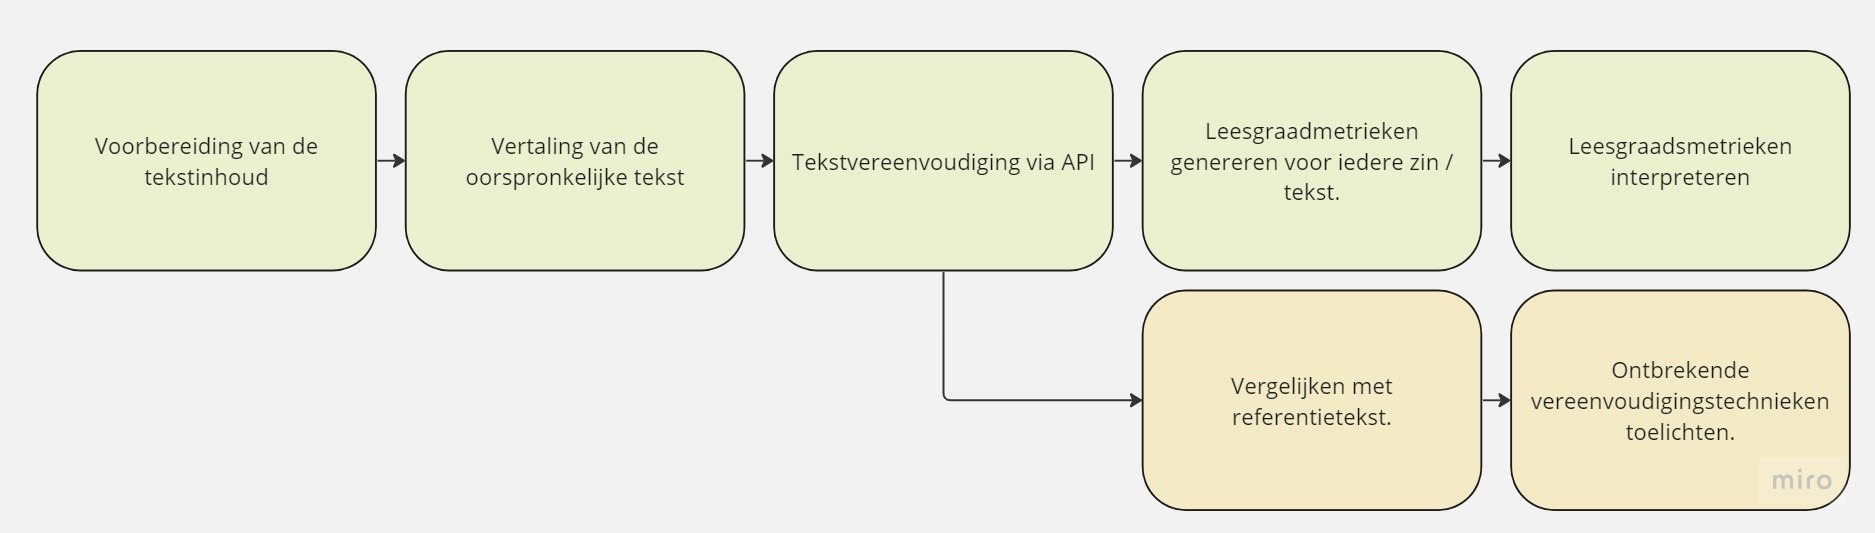
\includegraphics[width=\linewidth]{img/flowchart-vergelijkende-studie.jpg}
\caption{Flowchart voor het interpreteren van de }
\label{img:flowchart-vergelijkende-studie-metrics}
\end{figure}

\medspace 

De referentieteksten zijn geschreven door twee leerkrachten binnen het vakgebied onderwijs, en twee scholieren van de derde graad in het middelbaar onderwijs zonder dyslexie. Deze vier personen baseren zich op vooraf meegekregen richtlijnen, toegelicht in de bijlage. 

\medspace



\medspace

% SCRIPT 1
Eerst volgt er een voorbereiding van de tekstinhoud. Hier wordt namelijk de inhoud van de wetenschappelijke artikelen opgehaald, en vervolgens in een tekstbestand geplaatst. Dit gebeurt manueel. Dit gebeurt met de code verwezen in \ref{code:verg-studie-phase-1}. Aangezien GPT-3 en de HuggingFace-taalmodellen enkel per commandline of Python-script werken, krijgt het taalmodel alle bruikbare testinhoud in \textit{plain-text}. Deze bruikbare tekstinhoud omvat alle tekst uit het wetenschappelijk artikel, met uitzondering op de bibliografie en inhoudsopgave.


% SCRIPT 2
Zoals eerder verwezen, moeten de taalmodellen via HuggingFace eerst vertaald worden naar Engelstalige tekst. Zo staat het vertalen in de tweede fase centraal, verwezen in script \ref{code:verg-studie-phase-2}. Aangezien het onderzoek probeert te werken met zo vaak mogelijk open-source of vrij beschikbare software, wordt er gebruik gemaakt van de \textit{deep\_translator} Python-bibliotheek. Het script itereert iedere zin en vertaalt de zin naar het Engels, indien dit een niet-Engelstalige zin is. Het resultaat van dit script is een csv-bestand met daarin twee kolommen, alle Nederlandstalige en alle vertaalde Engelstalige zinnen van één artikel. Bij een Engelstalig artikel bevatten de twee kolommen dezelfde waarden. De kolommen worden gesepareerd met een pipe-symbool.

\medspace

% SCRIPT 3
Vervolgens wordt iedere zin aan het taalmodel gegeven, zo om voor elke zin een vereenvoudigde versie te krijgen. T1 en T2 vereenvoudigen de Engelstalige zinnen, in tegenstelling tot T3 en de verwante prompts die de Nederlandstalige zin vereenvoudigen. Bij het schrijven van de prompt wordt er rekening gehouden met de verwachte \textit{output format}. 

Eerst worden de specifieke tokenizers en modellen van T1 en T2 gedeclareerd, alsook wordt de API-sleutel voor GPT-3 ingesteld. Het script itereert over alle tekstbestanden aangemaakt in fase 2 of in script \ref{code:verg-studie-phase-2}.


% Dit maakt het behandelen van niet-Engelstalige wetenschappelijke artikelen moeilijk. 

\medspace

Taalmodellen via HuggingFace worden lokaal opgezet en worden niet aangepast. Tabel \ref{table:tested-prompts} geeft de gebruikte prompts voor de testen bij het GPT-3 model weer. Zowel het Seq2Seq als het toegepaste GPT-3 model maken gebruik van een nul-temperature en een top-p waarde van 90\%, zo om een probabilisch vertrouwd antwoord te verkrijgen, alsook om een hoge woordfrequentie te bekomen, zoals eerder aangegeven in \ref{table:gpt-3-parameters}.

\medspace

Zoals eerder aangehaald kunnen prompt-gebaseerde testen verschillende resultaten bekomen, afhankelijk van de gegeven input. Daarom benadert de vergelijkende studie vijf verschillende prompts, gebaseerd op de verschillende tekstvereenvoudigingstechnieken beschreven in \ref{table:manual-simplification}. De tokenlengte kan een request doen falen. Daarom breekt het script de tekst per paragraaf op.

\begin{center}
	\begin{table}[H]
		\begin{tabular}{ | m{2cm} | m{14cm} | } 
			\hline
			\textbf{Naam} & \textbf{Prompt} \\
			\hline
			P1 & Vereenvoudig deze tekst \\
			\hline
			P2 & Vereenvoudig deze tekst voor studenten (16-18 jaar) door moeilijke woorden te vervangen, vakjargon te schrappen, woorden langer dan 18 letters te vervangen, acroniemen voluit te schrijven, een woord slechts eenmaal door een synoniem te vervangen, korte uitleg te geven wanneer dat nodig is, en percentages te vervangen. \\
			\hline
			P3 & Vereenvoudig een tekst door deze op te delen in kortere zinnen van maximaal tien woorden. Verander voornaamwoorden als 'zij', 'hun' of 'hij' in namen. Vervang complexe zinsconstructies en voorzetselzinnen door eenvoudiger alternatieven, maar laat ze ongewijzigd als er geen eenvoudiger optie beschikbaar is. \\
			\hline
		\end{tabular}
		\label{table:tested-prompts}
		\caption{De GPT-3-prompts die in de vergelijkende studie aan bod komen.}
	\end{table}
\end{center}


Leesgraadsformules dienen, zoals aangegeven in \textcite{Nenkova2004}, als objectieve maatstaf bij deze vergelijkende studie. De bekomen leesgraadmetrieken ondergaan een vergelijking met elkaar en met die van een referentietekst. De vergelijking gebeurt zowel subjectief als objectief aan de hand van de leesgraadsmetrieken benoemd in tabel \ref{table:readability-scores}. Code-blok \ref{code:script-for-text-analysis} past de Pandas-bibliotheek in combinatie met de Readability-library toe om een CSV te maken met alle leescriteria.

\medspace

Naast leesgraadsmetrieken moeten de vereenvoudigde teksten eveneens de semantiek van de tekst kunnen behouden, alsook de volledige kern van de tekstinhoud nog steeds bijhouden. Zo moeten de referentieteksten capabel zijn om alle meegegeven vragen te beantwoorden.

\medspace

De vergelijkende studie bepaalt welk taalmodel nodig is om gepersonaliseerde tekstvereenvoudiging in het prototype aan te bieden, nadrukkelijk om wetenschappelijke artikelen met ATS te vereenvoudigen op maat voor scholieren met dyslexie in de derde graad van het middelbaar onderwijs en met een vergelijkbare kwaliteit als een vereenvoudiging met MTS. 








\section{Prototype voor tekstvereenvoudiging}

Met de benodigde functionaliteiten en de geschikte taalmodel voor gepersonaliseerde ATS, kan het onderzoek een volgende stap zetten richting de onderzoeksvraag. Deze sectie omschrijft de ontwikkeling van een prototype voor gepersonaliseerde tekstvereenvoudiging voor scholieren met dyslexie in de derde graad van het middelbaar onderwijs en geeft daarmee een antwoord op de volgende deelvraag: 

\begin{itemize}
	\item Hoe kan een intuïtieve en lokale webtoepassing worden ontwikkeld die zowel scholieren met dyslexie als docenten helpt bij het vereenvoudigen van wetenschappelijke artikelen met behoud van semantiek, jargon en zinsstructuren?
\end{itemize}

Allereerst moeten de gebruikte technologieën benadrukt worden. Eerdere onderzoeken maakten sporadisch gebruik van Python-technologieën en dit prototype volgt deze voorafgaande onderzoeken en vakliteratuur. Tabel \ref{table:technologies} geeft een breed overzicht van alle gebruikte programmeertalen. Hierop vult tabel \ref{table:python-libraries} aan door een overzicht te geven van alle gebruikte Python-libraries.

\begin{center}
	\begin{table}[H]
	\begin{tabular}{ | m{4cm} | m{12cm} | } 
		\hline
		\textbf{Technologie} & \textbf{Functionaliteit} \\
		\hline
		Python & De back-end van het prototype die API-calls en de NLP-functionaliteiten zoals PoS-tagging en lemmatizing verwerkt. \\
		\hline
		JavaScript & De toepassing gebruikersvriendelijker maken, personalisatie-opties voor de site doorvoeren en de functies gebouwd in Javascript dienen als alternatief op commandline instructies. \\
		\hline
		HTML en CSS & Het visuele uiterlijk van de website aanpassen naargelang de gekozen parameters van de eindgebruiker. \\
		\hline
		Jinja & Informatie uit de back-end (Python) doorgeven aan de front-end (JavaScript).  \\
		\hline
		Docker & Lokale uitrol van de webtoepassing. \\
		\hline
		Bash & Intuïtief script om de webtoepassing op te starten voor Linux en Mac-systemen. \\
		\hline
		Powershell & Intuïtief script om de webtoepassing op te starten op Windows-systemen. \\
		\hline
	\end{tabular}
	\label{table:technologies}
	\caption{Gebruikte programmeertalen in het prototype voor tekstvereenvoudiging.}
	\end{table}
\end{center}

\begin{center}
	\begin{table}[H]
	\begin{tabular}{ | m{4cm} | m{12cm} | } 
		\hline
		\textbf{Python-bibliotheek} & \textbf{Functionaliteit} \\
		\hline
		Flask					& Het framework van de webtoepassing. Deze combineert front-end en back-end en past binnen de scope van een prototype. \\ % later kan dan geopteerd worden voor een aparte front-end en back-end
		\hline
		PDFMiner 				& Tekstinhoud van PDF's inlezen. \\ 
		\hline
		EasyOCR					& PDF-pagina's inscannen als afbeelding in JPG-formaat om vervolgens de tekst te extraheren. \\
		\hline
		NumPy 					& De reshape-functie vereenvoudigt de manier om arrays van zinnen bij elkaar te plaatsen om zo een paragraaf te bekomen. \\
		\hline		
		Spacy 					& PoS-tagging en het lemmatiseren van woorden. \\
		\hline
		OpenAI					& GPT-3 API aanspreken. \\
		\hline
		Requests				& HuggingFace API aanspreken en informatie ophalen van een lexicale databank API. \\
		\hline
		BeautifulSoup			& HTML-content \textit{parsen} zodat de aangepaste inhoud van een leerkracht correct geformatteerd kan worden naar een PDF. \\
		\hline
	\end{tabular}
	\label{table:python-libraries}
	\caption{Gebruikte Python-libraries en hun respectievelijke functie in het prototype.}
	\end{table}
\end{center}

\medspace

De homepagina, weergegeven op figuur \ref{img:homepage}, biedt een kort overzicht van de twee algemene functionaliteiten, alsook instellingen waar gebruikers de webtoepassing kunnen aanpassen naargelang hun voorkeuren. Zoals aangeraden in \ref{ch:stand-van-zaken} door \textcite{Harvard2023}, moeten ontwikkelaars reking houden met de personalisering van de website. Deze functionaliteit gaat volgens hem vaak onopgemerkt en heeft nochtans een bewezen effect op het leesgedrag -en begrip van zowel mensen met als zonder dyslexie. De webtoepassing maakt gebruik van de standaardparameters, uitgewezen in \textcite{Rello2013a, Rello2013b}. Op een apart scherm kan de eindgebruiker de volgende elementen aanpassen naar hun toebehoren. Het prototype kan na aanpassing van de parameters eruit zien zoals weergegeven in figuur \ref{img:website-instellingen}. JavaScript maakt het mogelijk om deze parameters dynamisch en on-the-spot aan te passen. Na een aanpassing zal de back-end de sessievariabelen aanpassen naargelang de gekozen parameters, zodat de eindgebruiker niet per pagina deze parameters moet instellen. Voor dit prototype zijn er twee soorten eindgebruikers: leerkrachten die wetenschappelijke artikelen met ATS willen vereenvoudigen op maat van scholieren en de scholieren die dit zelf willen doen. Beide doelgroepen hebben hun eigen noden, maar toch een centraal doel voor ogen: het gepersonaliseerd vereenvoudigen van een wetenschappelijk artikel.


\begin{center}
	\begin{figure}[H]
		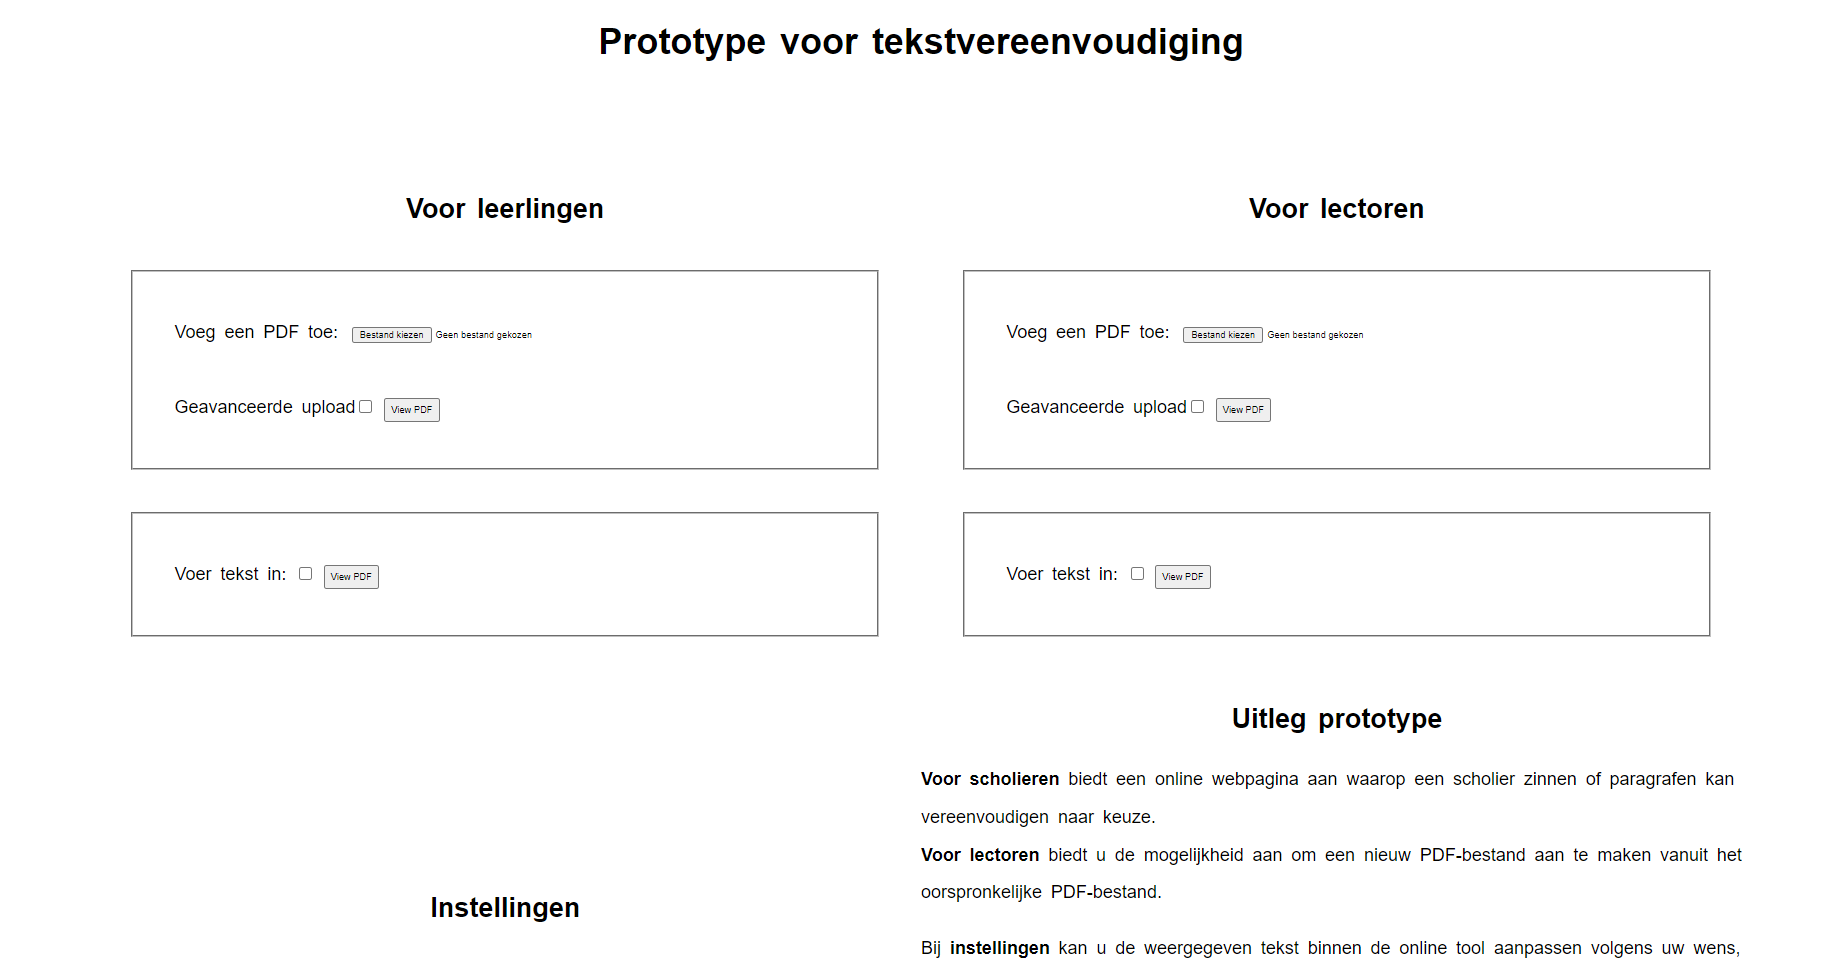
\includegraphics[width=\linewidth]{img/proto-homescreen.png}
		\caption{Een mogelijke weergaven van de homepagina.}		
		\label{img:homepage}
	\end{figure}
\end{center}

\begin{center}
	\begin{figure}[H]
		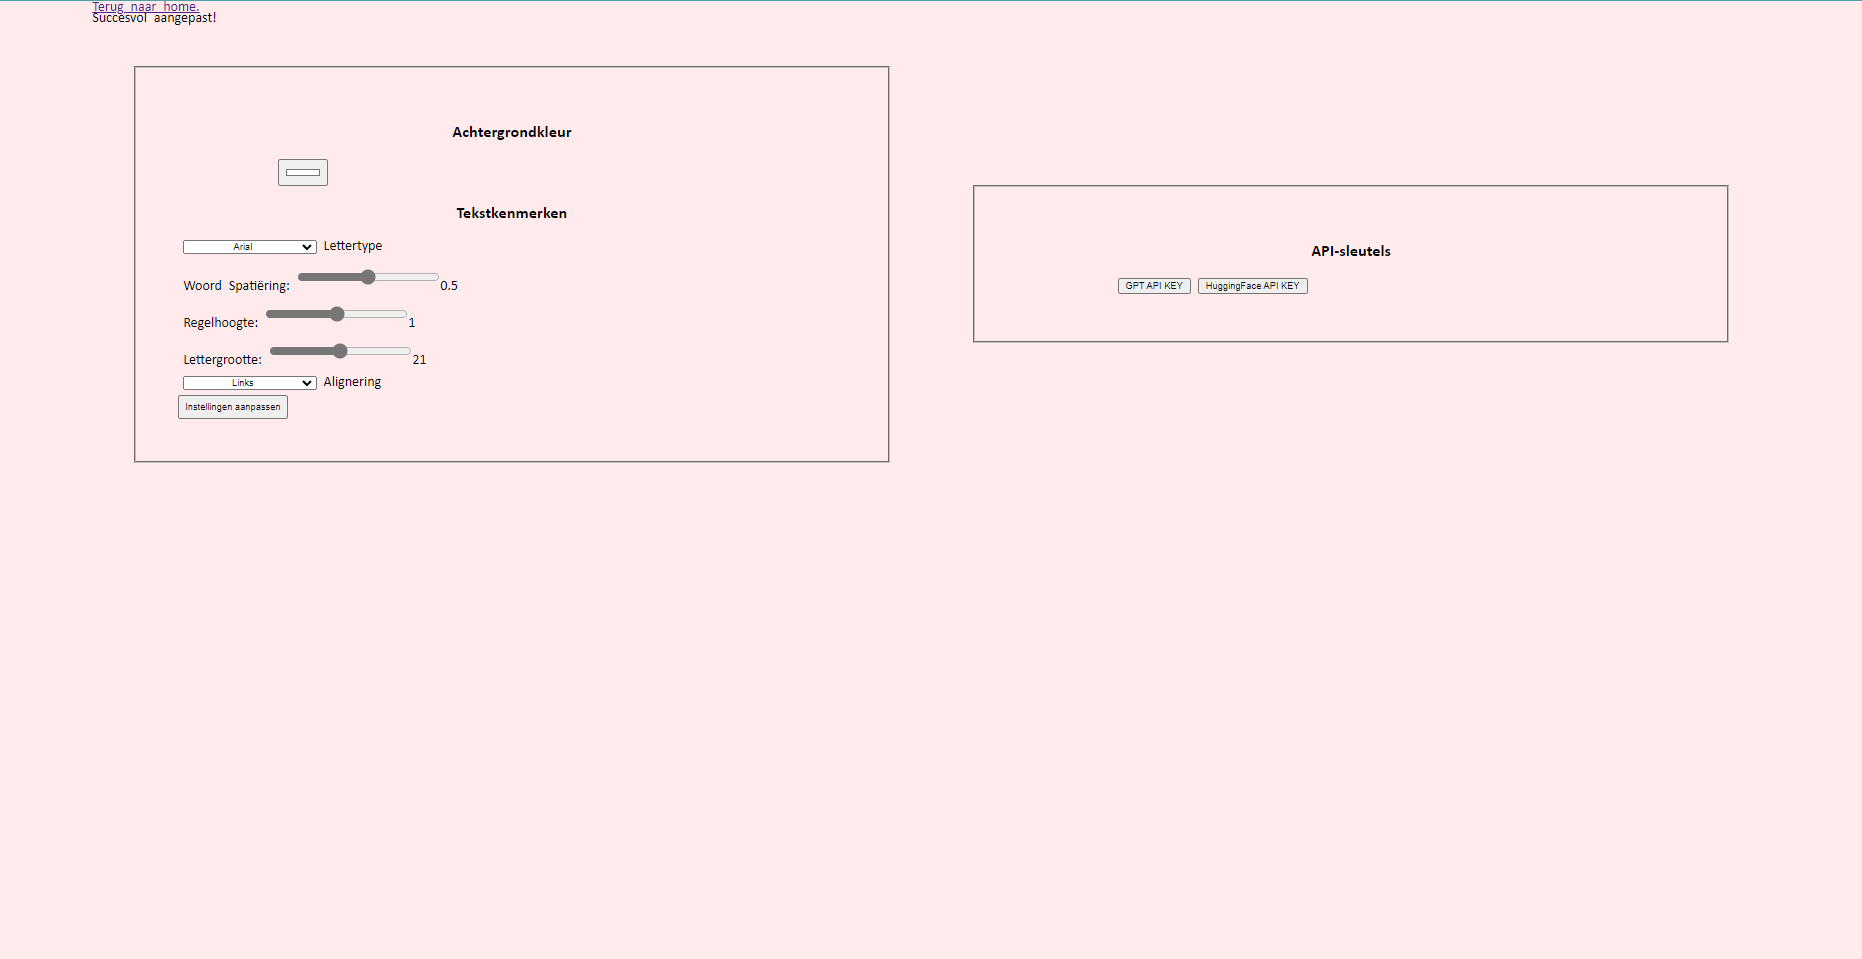
\includegraphics[width=\linewidth]{img/website-instellingen.png}
		\caption{Voorbeeldweergave van de instellingenpagina.}
		\label{img:website-instellingen}
	\end{figure}
\end{center}

De invoer van een wetenschappelijk artikel gebeurt voor beide doelgroepen op identieke wijze. De gebruiker kan een PDF of een stuk \textit{plain-text} ingeven als invoer van het wetenschappelijk artikel. Eindgebruikers kunnen met het prototype wetenschappelijke artikelen op één van twee manieren inladen: \textit{plaintext} of via een PDF-bestand. PDF's worden tijdelijk \textit{in-memory} opgeslaan. Daarmee kan het systeem niet na lange duur overbelast raken. Het prototype past eenzelfde functie toe om wetenschappelijke artikelen in te lezen voor de twee verschillende doelgroepen. Vooraf controleert de Flask-applicatie het type invoer. Vervolgens spreekt de Flask back-end de Reader-klasse aan die de tekst verder zal formatteren tot een bruikbaar formaat voor de webtoepassing. PDF extractors, waaronder PDFMiner, kunnen tekstinhoud verliezen tijdens het extraheren zoals eerder aangewezen in tabel \ref{sec:requirementsanalyse}. Als vangnet biedt het prototype een tweede optie aan waarbij de PDF-pagina's als afbeelding worden opgeslaan. Er wordt rekening gehouden met de splitsing tussen normale en geavanceerde upload. Deze twee methoden zijn terug te vinden in de Reader-klasse\footnote{https://github.com/Dyashen/text-simplification-tool/blob/main/web-app/Reader.py} ofwel bijlage \ref{code:reader-klasse}.

\begin{enumerate}
	\item PDFMiner itereert doorheen de PDF en extraheert vervolgens de tekst op iedere pagina. Deze methode resulteert in een string-object.
	\item De Python-bibliotheek EasyOCR voorziet een eenduidige en ontwikkelaarsvriendelijke manier om PDF-pagina's op te slaan als JPG of PNG. Tesserat biedt een even eenduidige oplossing aan, maar vergt meer configuraties en daarmee vergroot de omvang van de Docker-container. Vervolgens worden de afbeeldingen per text-chunk ingelezen en nadien opgeslaan. Het gebruik van deze alternatieve methode kan de omvang van de Docker-container vergroten. Om dit te voorkomen, verwijdert het prototype afbeeldingen nadat deze de tekstinhoud hebben geëxtraheerd en opgeslaan om zo ruimte te besparen. Net zoals bij de eerste methode resulteert deze methode in een string-object.
\end{enumerate}

De eerste fase van het prototype slaat de tekstinhoud op in meerdere arrays die zinnen voorstellen. Zoals aangegeven in \ref{code:reader-klasse}, staat de standaardparameter voor het aantal zinnen per paragraaf ingesteld op vijf zinnen, maar kunnen gebruikers aanpassen via het HTML-formulier bij de instellingen. Om de PoS-tag bij het respectievelijke woord bij te houden, maakt het prototype gebruik van een \textit{key-value pair} datastructuur. Zo verwijst de sleutel naar het woord in een zin; de waarde verwijst naar de PoS-tag die aan het woord toebehoord. Het prototype is enkel ontworpen voor Nederlandstalige en Engelstalige wetenschappelijke artikelen. Daarmee laadt het enkel twee embeddingsmodellen van Spacy op, zoals vermeldt in tabel \ref{table:wordembeddings-spacy}. Hardcoderen is uit den boze en daarom maakt het prototype gebruik van een \textit{dictionary} die de naam van deze embeddingsmodellen bijhoudt, zoals aangegeven in \ref{code:reader-klasse}. Zo is het systeem en hoeft er enkel een taalherkenning plaats te vinden. Fouttolerantie aanbieden gebeurt in de vorm van een standaardtaal in de dictionary, namelijk het Nederlands, of door vooraf de gebruiker te vragen in welke taal de opgelade tekst staat via een HTML-formulier.

% Deze transformatie bevoordeelt het proces om vervolgens de teksten per zin op de webpagina uit te printen. Bovendien is het manipuleren van het aantal zinnen per paragraaf een bewezen effect om de leesbaarheid van een tekst te verbeteren. 

\begin{center}
	\begin{table}
		\begin{tabular}{ | m{4cm} | m{12cm} | } 
			\hline
			\textbf{Taal} & \textbf{Embeddingsmodel} \\
			\hline
			Nederlands & NL Core News Medium\footnote{https://github.com/explosion/spacy-models/releases/tag/nl\_core\_news\_md-3.5.0} \\ 
			\hline
			Engels & EN Core Web Medium\footnote{https://github.com/explosion/spacy-models/releases/tag/en\_core\_web\_md-3.5.0} \\
			\hline
		\end{tabular}
		\label{table:wordembeddings-spacy}
		\caption{Gebruikte SpaCy Word-embeddings}
	\end{table}
\end{center}


\subsection{Tool voor leerkrachten}

In de vorm van een HTML-formulier kunnen leerkrachten gepersonaliseerde ATS met dit prototype waarmaken. Op de overzichtspagina kunnen leerkrachten beschikken over de functionaliteiten, weergegeven in tabel \ref{table:functionaliteiten-leerkrachten}. Het HTML-formulier omvat alle benodigde tekstvereenvoudigingstechnieken op lexicaal en syntactisch niveau die \ref{table:criteria-requirementsanalysis} verder uitwees. 

\begin{center}
	\begin{table}
		\begin{tabular}{ | m{7cm} | m{7cm} } 
			\hline
			\textbf{Functionaliteit} & Gebruikte JS/Python-techniek \\
			\hline
			Specifieke meegeven per paragraaf & Naast een optie om voor het hele document één prompt te gebruiken, voegt het prototype ook een optie toe om. Hiervoor past de web-inhoud een key-value structuur toe. \\
			\hline
			Opties voor gepersonaliseerde ATS aangeven. & Met behulp van een HTML-formulier kunnen leerkrachten checkboxes afvinken waaraan de gegenereerde tekst moet voldoen. Deze verschillende opties zijn terug te vinden in \ref{table:criteria-requirementsanalysis}. \\
			\hline
			Werkwoorden, bijvoeglijke en zelfstandige naamwoorden markeren & Front-end aanpassing met eventlistener. De tekstkleur van het aangeduide type woorden verandert naar het gekozen kleur. \\
			\hline
			Zinnen verwijderen & Front-end filter aangesproken door een \textit{eventlistener}. \\
			\hline
			Woord toevoegen aan woordenlijst & Een eventlistener handelt de functionaliteit af door de woorden en hun zin van voorkomen tijdelijk op te slaan in een storage. Het formulier houdt dit bij en geeft het vervolgens mee bij het indienen. Deze woorden en hun respectievelijke zin van voorkomen dienen om de woordenlijst op te vullen in het gegenereerde PDF of Word-bestand.\\ 
			\hline
			API-sleutel en sessieherkenning & Detectie met JS of een sessievariabele bestaat.
			\hline 
		\end{tabular}
	\label{table:functionaliteiten-leerkrachten}
	\caption{Alle beschikbare functionaliteiten in }
	\end{table}
\end{center}



\medspace

Om afwijkende resultaten op een GPT-prompt te vermijden, wordt de temperature op nul geplaatst en de \textit{top\_p} waarde wordt ingeschat op 80\%. SpaCy wordt gebruikt om woordkenmerken zoals de PoS-tag op te halen, maar het systeem is vatbaar voor het niet kunnen vinden van afwisselende en meertalige woordenschat. Een mogelijke oplossing is om de taal te veranderen naar Engels of Frans, of een aangepast taalherkenningsmodel te gebruiken. Een andere optie is om de tekst voor te verwerken om de Nederlandse en Engelse woorden te scheiden voordat ze worden verwerkt met SpaCy. Adjectieven uit de tekst verwijderen is mogelijk zonder taalmodel. Aangezien alle woorden gekoppeld worden aan een PoS-tag, is het eenvoudig om de woorden gelinkt aan de span-tag van de adjectieven uit te filteren.

\medspace

De eenduidige HTML-structuur van online woordenboeken maken het mogelijk om gratis en eenvoudig de definities van woorden op te halen. Zo is het mogelijk om annotaties op te halen zoals aangewezen in het onderzoek van \textcite{Bulte2018}. Met behulp van Requests en BeautifulSoup is het mogelijk om lijsten met definities te scrapen van deze sites. De stam van het gemarkeerde woord wordt opgehaald en vervolgens meegegeven als zoekopdracht. De bron wordt samen met het resultaat aan de eindgebruiker getoond. 

\subsubsection{Tekstvereenvoudiging}

Het prototype gebruikt een taalmodel van \textit{HuggingFace} voor extraherende samenvattingen en zowel gratis taalmodellen van \textit{HuggingFace} als het GPT-3 taalmodel voor abstraherende samenvattingen. Het model kan parameters, zoals maximale lengte van de gegenereerde tekst, ontvangen en biedt zowel gepersonaliseerde als niet-gepersonaliseerde vereenvoudiging. Het gebruik van \textit{HuggingFace} vereist een internetverbinding en kan geen extra trainingsdata bevatten. De opstarttijd voor alle \textit{HuggingFace}-taalmodellen wordt bij de start van de applicatie afgehandeld door middel van een extra parameter de request. Sleutels worden standaard bijgehouden in env-bestanden. Via de webtoepassing kan een gebruiker deze sleutel aanpassen. Binnen een lokale omgeving is dit in orde, al moeten ontwikkelaars rekening houden met beveiligingsmaatregelen wanneer een dergelijke tool wordt uitgerold. Het merendeel van de gebruikte taalmodellen is Engelstalig of is nadrukkelijk getraind op basis van Engelstalige datasets. De ingegeven tekst wordt eerst vertaald naar het Engels om zo de kans op een accurate vereenvoudiging te verhogen. Voor de vertaling wordt de Google Translate Python-package gebruikt. Deze is minder accuraat vergeleken met DeepL, maar biedt een gratis beschikbaar en aanvaardbaar alternatief aan. Factoren zoals topic diversity en semantische redundantie moeten overwogen worden bij het kiezen van een taalmodel voor extraherend samenvatten. Lange documenten samenvatten kan zoals aangeduid in literatuurstudie door extraherende samenvatting, gevolgd door abstraherende samenvatting om de tekst coherent te doen blijken. Eerder werd er gekozen om de voltekst per paragraaf bij te houden. Uit iedere paragraaf wordt een ideaal aantal zinnen gemarkeerd om nadien geparafraseerd te worden door GPT-3 of een \textit{HuggingFace} taalmodel, afhankelijk van de keuze van de eindgebruiker.


% TODO GPT-3

transformeren de tekst op lexicaal en syntactisch niveau. Zij bekijken enkel de gekregen zin. Andere taalmodellen zijn eerder geneigd om extra tekst toe te voegen. Er kan niet achterhaald worden waarom dat deze extra tekst wordt meegegeven. BART-SC kan bijzaak behouden, terwijl SC sneller de neiging heeft om enkel de kernzaak te behouden in de vereenvoudigde tekst. 

Bij de inference API van T1 moet er expliciet worden aangegeven om welke transformatie dit gaat door kernwoorden zoals 'simplify:'.

\medspace

De zelfgebouwde Creator-klasse bouwt PDF's en docx-documenten op volgens de meegegeven personalisatie. Het prototype maakt gebruik van Pandoc, of PyPandoc via Python. Pandoc maakt gebruik van een tweestapsbeweging, waarbij plain-text eerst naar een Markdown-formaat wordt omgezet om vervolgens het Markdown-bestand naar een PDF of Word document te converteren.

\medspace

Met Python wordt eerst een YAML-header in het te-transformeren Markdown-bestand geschreven. De YAML-header omvat de titel, standaardlettertype en lettertype voor de titel, de datum, het type document dat moet worden gegenereerd, de marge-instelling, de standaardlettergrootte, woord-spatiëring en ten slotte de instelling voor de regeleinde. De meegekregen gepersonaliseerde instellingen wordt meegegeven in een LateX YAML-header.

\medspace

De structuur om de woordenlijst op te bouwen, is identiek zoals dat van een Markdown-tabel. De  woordenlijst wordt in dictionary-structuur meegegeven. De sleutels worden overlopen en vervolgens wordt ieder woord samen met de PoS-tag en de definitie uitgeprint. De vereenvoudigde tekst is eveneens in een dictionary-structuur opgeslaan. De keys stellen titels voor en worden uitgeprint voorafgegaan door twee hekje-symbolen. Tussen de titels worden breaklines toegevoegd, gevolgd door de tekst die bij de titel bijhoort. Indien gekozen werd voor een opsomming, dan wordt er gebruik gemaakt van een geneste for-lus waarbij iedere zin wordt voorafgegaan aan een asterisk-symbool. De woordenlijst en vereenvoudigde tekst worden naar hetzelfde Markdown-bestand uitgeschreven. 

\medspace

Als invoer wordt het pad naar opgevulde Markdown-bestand meegegeven. De uitvoer is het pad waarnaar het PDF- of DOCX-bestand moet worden opgeslaan. Vervolgens zet Pandoc het Markdown-bestand om naar een PDF-bestand gebouwd met de XeLateX engine of een Word-bestand op basis van meegekregen binaries. Pandoc Flask kan enkel één bestand aan de gebruiker teruggeven. Als oplossing comprimeert het prototype met \textit{zipfile} de PDF- en Wordbestand tot één bestand. 

\begin{figure}[H]
	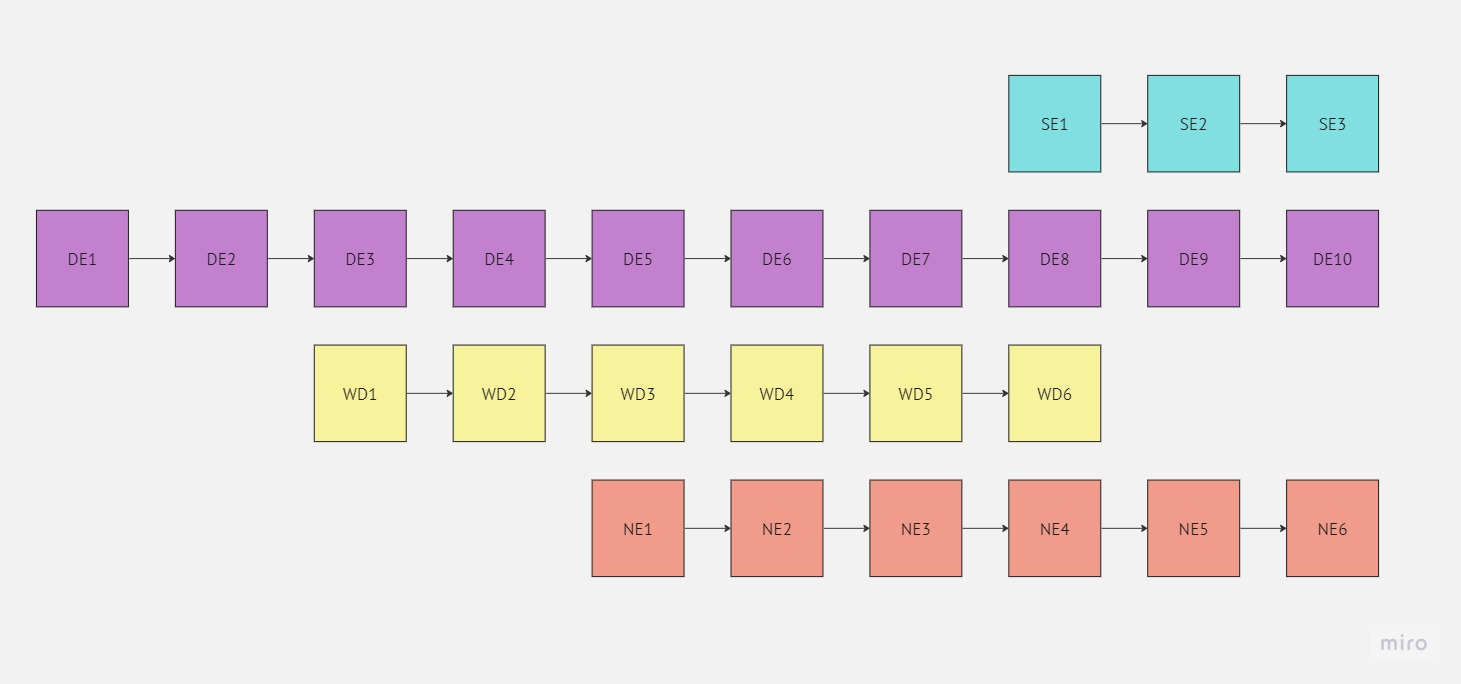
\includegraphics[width=\linewidth]{img/flowchart-development.jpg}
	\caption{Stappenplan voor de ontwikkeling van het component voor lectoren.}
	\label{img:stappenplan-leerkrachten}
\end{figure}

\begin{center}
	\begin{table}
		\begin{tabular}{ | m{2cm} | m{12cm} | } 
			\hline
			WD1 & Flask-skelet aanmaken \\
			WD2 & Formulier voor GPT-3 API-sleutel invoer maken + sessie \\
			WD3 & Formulier voor gepersonaliseerde opties van website aanmaken + sessie \\
			WD4 & Webpagina's aanmaken in HTML \& CSS \\
			WD5 & Invoerformulier maken voor PDF- en tekstupload \\
			WD6 & Invoerformulier maken voor het genereren van een gepersonaliseerde vereenvoudiging van een wetenschappelijk artikel \\
			\hline
		\end{tabular}
		\label{table:tasks-web-engineer}
		\caption{Taken van de webontwikkelaar bij het uitwerken van het lerarencomponent.}
	\end{table}
\end{center}

\begin{center}
	\begin{table}[H]
		\begin{tabular}{ | m{2cm} | m{12cm} | } 
			\hline
			NE1 & Spacy word embeddings laden \&PoS-tagging en lemmatization implementeren \\
			NE2 & Dictionary implementen voor het bijhouden van de PoS-tag per dictionary \\
			NE3 & Jupyter notebook om gepersonaliseerde prompts en aangepaste hyperparameters uit te testen voor de GPT-3 API \\
			NE4 & Jupyter notebook gebruiken om tekstvereenvoudigingsfuncties met GPT-3 API uit te testen. \\
			NE5 & Optioneel: Extra trainingsdata toevoegen aan GPT-3 model. \\
			NE6 & Code voor de voorgestelde pipeline voor ATS implementeren in Python back-end. \\
			\hline
		\end{tabular}
		\caption{Taken van de NLP Engineer bij het uitwerken van het lerarencomponent.}
		\label{table:tasks-nlp-engineer}
	\end{table}
\end{center}


\begin{center}
	\begin{table}[H]
		\begin{tabular}{|m{2cm}|m{12cm}|}
			\hline
			DE1	& Python-notebook om PDFMiner uit te testen bij willekeurige wetenschappelijke artikelen (2000 - nu) \\
			DE2 & Python-notebook opstellen om EasyOCR uit te testen bij willekeurige wetenschappelijke artikelen \\
			DE3 & Jupyter notebook om tekstdata cleaning te realiseren. De restanten van de PDF-extractie moeten weg. \\
			DE4 & Jupyter notebook om look-up methode voor synoniemen te realiseren. \\
			DE5 & Code in back-end implementeren voor PDF-upload via in-memory PDF read. \\
			DE6 & Python-notebook om Pandoc PDF \& Word-document te genereren. \\
			DE7 & Uittesten van YAML-header in Markdown-bestand voor een document op maat. \\
			DE8 & Uittesten van uitschrijven tekstinhoud naar Markdown-bestand \\
			DE9 & Implementatie code van Pandoc in Flask-framework \\
			DE10 & Code in back-end implementeren voor zippen \& doorsturen naar eindgebruiker. \\
			\hline
		\end{tabular}
			\caption{Taken van data engineer bij het uitwerken van het lerarencomponent.}
			\label{table:tasks-data-engineer}
	\end{table}
\end{center}

\begin{center}
	\begin{table}
		\begin{tabular}{|m{2cm}|m{12cm}|}
			\hline
			SE1 & Dockerfile en bijhorende requirementsfile aanmaken \\
			SE2 & Opzet in Docker realiseren \\
			SE3 & Powershell en Bash-script realiseren \\
			\hline
		\end{tabular}
		\label{table:tasks-system-engineer}
		\caption{Taken van de system engineer bij het uitwerken van het lerarencomponent.}
	\end{table}
\end{center}


\subsection{Tool voor scholieren}

De taken van de NLP engineer blijven vrijwel dezelfde, dus hier wordt er verwezen naar de taken in tabel \ref{table:tasks-nlp-engineer}. De taken van de systeemingenieur vallen in dezelfde lijn als die bij het lerarencomponent, dus ook hier wordt er verwezen naar de taken beschreven in tabel \ref{table:tasks-system-engineer}. De bijhorende flowchart wordt weergegeven in figuur \ref{img:stappenplan-scholars}.

\medspace

De weergave van de tool voor scholieren oogt gelijkaardig aan dat van de uitgeteste chatbots. Figuur \ref{ } geeft een blik op hoe de webpagina er kan uitzien bij start. Met JavaScript kunnen de volgende functionaliteiten aangeboden worden:

\begin{center}
	\begin{table}
		\begin{tabular}{cols}
			\hline
			Functionaliteit & JavaScript-functie & Python-functie \\
			\hline
			
			\hline
		\end{tabular}
	\end{table}
\end{center}

\begin{figure}[H]
	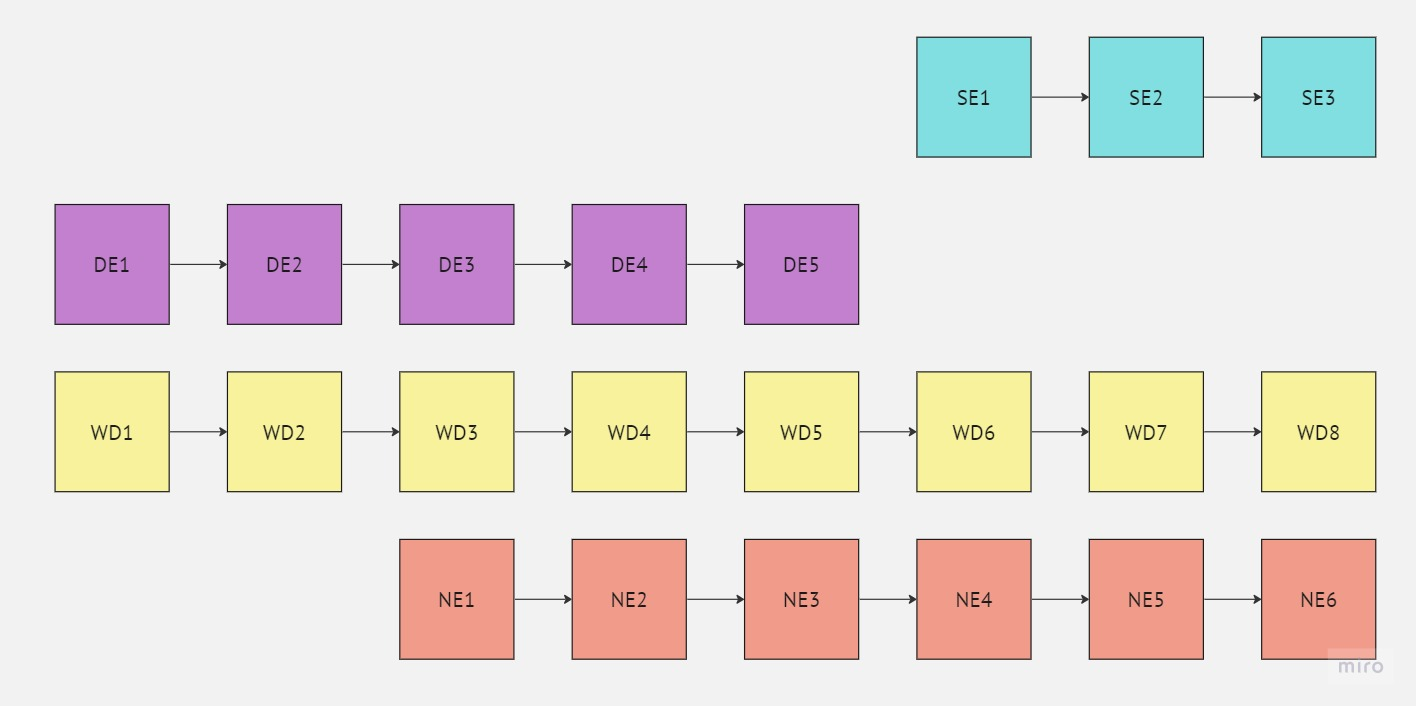
\includegraphics[width=\linewidth]{img/flowchart-development-scholars.jpg}
	\caption{Stappenplan voor de ontwikkeling van het component voor scholieren.}
	\label{img:stappenplan-scholars}
\end{figure}

\begin{center}
	\begin{table}
		\begin{tabular}{ | m{2cm} | m{12cm} | } 
			\hline
			WD1 & Flask-skelet aanmaken \\
			WD2 & Formulier voor GPT-3 API-sleutel invoer maken + sessie \\
			WD3 & Formulier voor gepersonaliseerde opties van website aanmaken + sessie \\
			WD4 & Webpagina's aanmaken in HTML \& CSS \\
			WD5 & Invoerformulier maken voor PDF- en tekstupload \\
			WD6 & JavaScript-functies schrijven voor het weergeven van grammaticale structuren, bijvoeglijke en zelfstandige naamwoorden. \\
			WD7 & JavaScript functies schrijven voor dynamische tekstaanpassing met placeholder-tekst \\
			WD8 & API-calls schrijven voor de functies: look-up, lexicale vereenvoudiging, formaatwijzigingen en ten slotte prompt-gedreven tekstvereenvoudiging \\
			\hline
		\end{tabular}
		\caption{Taken van NLP engineer bij het uitwerken van het scholierencomponent.}
		\label{table:tasks-nlp-engineer-scholars}
	\end{table}
\end{center}

\begin{center}
	\begin{table}[H]
		\begin{tabular}{|m{2cm}|m{12cm}|}
			\hline
			DE1	& Python-notebook om PDFMiner uit te testen bij willekeurige wetenschappelijke artikelen (2000 - nu) \\
			DE2 & Python-notebook opstellen om EasyOCR uit te testen bij willekeurige wetenschappelijke artikelen \\
			DE3 & Jupyter notebook om tekstdata cleaning te realiseren. De restanten van de PDF-extractie moeten weg. \\
			DE4 & Jupyter notebook om look-up methode voor synoniemen te realiseren. \\
			DE5 & Code in back-end implementeren voor PDF-upload via in-memory PDF read. \\
			\hline
		\end{tabular}
		\caption{Taken van data engineer bij het uitwerken van het scholierencomponent.}
		\label{table:tasks-data-engineer-scholars}
	\end{table}
\end{center}

\medspace

Ten slotte maakt het prototype gebruik van Docker voor de lokale opzet. Een scriptbestand, in Powershell of Bash, vereenvoudigt de opstart van deze webapplicatie, in tegenstelling tot de opstart per terminal. Alvorens installeert Docker met behulp van de voorafgegeven instructies de nodige Python-bibliotheken met het Pipreq-commando. Omdat het prototype gebruik maakt van de API's van de taalmodellen, hoeft het prototype geen gebruik te maken van een aparte container voor het taalmodel.

% Ontwikkelaars moeten rekening houden met het gebrek aan structuur bij het ophalen van tekstinhoud uit een PDF-bestand.